
\begin{frame}
		\begin{figure}
				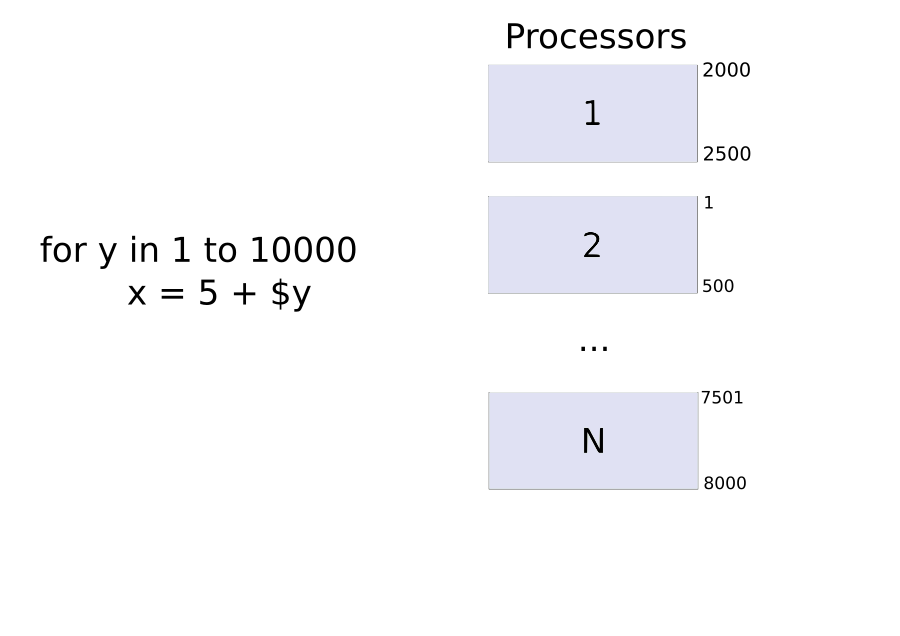
\includegraphics[width=0.8\linewidth]{figures/diagrams/forloop/fordiagram}
		\end{figure}	
\end{frame}

\begin{frame}
		\begin{figure}
				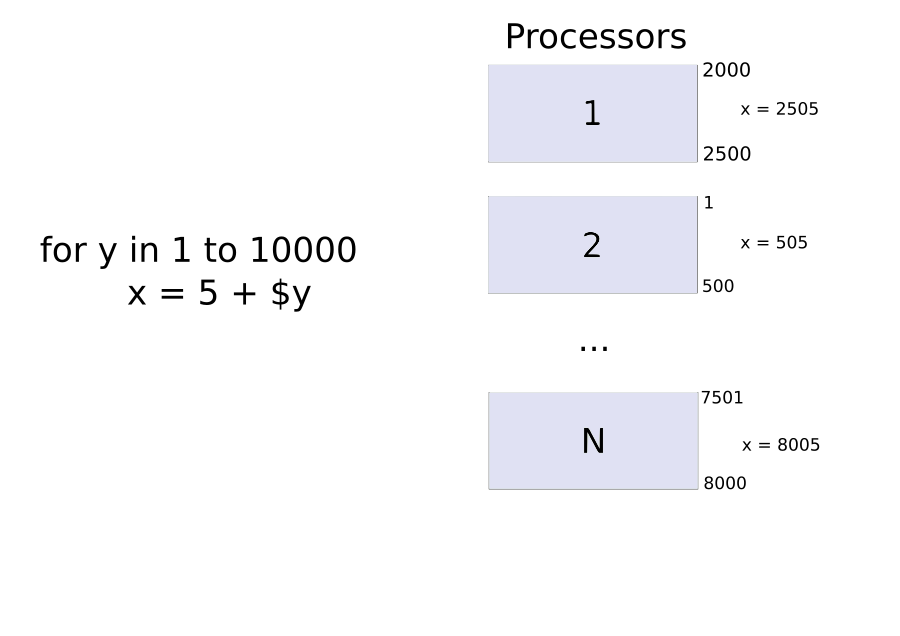
\includegraphics[width=0.8\linewidth]{figures/diagrams/forloop/fordiagram2}
		\end{figure}	
\end{frame}

\begin{frame}
		CLI examples of parallel utilities
\end{frame}


\begin{frame}[fragile]
		\frametitle{R parallel package}
		\center
		\begin{verbatim}
			library(doParallel)
			cl <- makeCluster(2)
			registerDoParallel(cl)
			foreach(i=1:3) %dopar% sqrt(i)
		\end{verbatim}
\end{frame}

\begin{frame}
		observed/expected speedup (figure)
\end{frame}

\begin{frame}
		Amdahl's law (code diagram)
\end{frame}

\begin{frame}
		Parallelization overhead (code diagram)
\end{frame}

